% TEMPLATE for Usenix papers, specifically to meet requirements of

% https://www.usenix.org/conference/usenixsecurity17/submitting-papers

% Complaints to /dev/null.
% This version uses the latex2e styles, not the very ancient 2.09 stuff.
\documentclass[letterpaper,twocolumn,10pt]{article}
\usepackage{lib/usenix,epsfig,endnotes,tabularx}
\begin{document}

%don't want date printed
\date{}

%make title bold and 14 pt font (Latex default is non-bold, 16 pt)
\title{\Large \bf One-Step, Three-Factor Authentication With Custom-Fit, In-Ear EEG}

%forsupose single author (just remove % characters)
\author{
{\rm First Name, Second Name, Third Name}\\
First Institution
\and
{\rm Second Name}\\
Second Institution
% copy the following lines to add more authors
% \and
% {\rm Name}\\
%Name Institution
} % end author

\maketitle

% Use the following at camera-ready time to suppress page numbers.
% Comment it out when you first submit the paper for review.
\thispagestyle{empty}


\subsection*{Abstract}
In this paper, we present a system that provides all three factors of authentication (knowledge, possession, and inherence) in a single step, using brain-based authentication via a custom-fit, in-ear EEG. Across all participants, we achieve mean 0\% false acceptance and 0.12\% false rejection rates with data from only one earpiece with three electrodes. We find a 0\% false acceptance rate in a preliminary simulation of an impersonation attack. Our results indicate that in-ear EEG could provide a discreet, convenient, and useable means for one-step, multi-factor authentication.

\section{Introduction}
\label{sec:org7196b99}

It is well appreciated by experts and end-users alike that strong authentication is
critical to cybersecurity and privacy, now and into the future. Unfortunately,
news reports of celebrity account hackings serve as regular reminders that
the currently dominant method of authentication in consumer applications, 
single-factor authentication using passwords or other user-chosen secrets, 
faces many challenges. Major industry players such as Google and
Facebook have strongly encouraged their users to adopt two-factor
authentication (2FA). However, submitting two different 
authenticators in two separate steps has frustrated wide adoption
due to its additional hassle to users. The Apple iPhone, for instance,
already supports device unlock using either a user-selected passcode or a fingerprint. The
device could easily support a two-step two-factor authentication scheme if
desired. However, it is easy to understand why users would balk at having to
enter a passcode \emph{and} provide a fingerprint each time they want to unlock their phone.

In previous work, "one-step two-factor authentication" has been proposed as a
new approach to authentication that can provide the security benefits of two-
factor authentication without incurring the hassle cost of two-step verification.
By employing consumer-grade EEG (electroencephalogram),
it was demonstrated in a 2013 passthoughts study that a user can
submit both a knowledge factor (i.e., secret thought) and an inherence factor
(i.e., brainwave signal unique to the individual) in a single step by performing a
single mental task \cite{Chuang2014}. Additionally, the robustness of this method against
impersonation attacks was demonstrated, including conditions where the attacker
may have learned the target'��s secret thought and/or secret task \cite{Johnson2014}.

In this study we undertake, to the best of our knowledge, the first
ever study of one-step, three-factor authentication. In computer security,
authenticators are classified into three types: knowledge factors (e.g., passwords
and PINs), possession factors (e.g., physical tokens, ATM cards), and inherence
factors (e.g., fingerprints and other biometrics).

We find that we can achieve low FARs and FRRs with a single, three-electrode earpiece.
Interestingly, we found that performance improves in the ear compared to on the scalp.
Additionally, we find that an passthoughts could not be spoofed by imposters, even when the imposters had the subject's earpiece and knew the secret passthoughts.
We discuss the benefits of passthoughts to usable authentication, and raise questions about how and why passthoughts work as well as they do.

\section{Related work}

Because three-factor authentication (3FA) requires the user to
submit one distinct instance of each
type of authenticator, it represents the strongest level of authentication security
possible. The system we propose and test here uses the choice of a mental task
or "passthought" to perform as knowledge, the uniqueness of an individual's brain
activity as measured by EEG as inherence, and the physical token of custom-fit 
earpieces which could easily contain a hardware key-pair as a possession factor.
The ability to utilize all three of these security factors in a single step by performing 
a mental task of a few seconds is a promising in pursuit of extremely strong security 
while maintaining a low amount of effort and obtrusiveness to the user.

Following this work, we investigate custom-fit ear-EEG technology as the platform for
investigating the feasibility, performance, and usability of one-step three-factor
authentication. In addition to the dual knowledge and inherence factors in
in previous work, this work includes a possession factor
in the form of the EEG-sensing ear-piece(s) that are custom-fitted to and worn in
their ear. These earpieces can serve as physical tokens in the same way as bank
ATM cards and wearable hardware tokens by implementing a hardware key-pair.
Furthermore, because the earpieces are custom-fitted to each individual, we predicted 
they would likely not be able to produce good electrical impedances when worn by a different individual.

\subsection{Usable authentication}

Authentication protocols are often susceptible to a so-called \textit{rubber-hose attack}, in which users are coerced into giving up their chosen secret (e.g. password), biometric, or unique token, voluntarily or not \cite{Bojinov2012, Martinovic2012}. This attack is particularly effective against protocols that rely only on inherence factors, as inherent traits such as fingerprints are difficult to change without costly reprocussions \cite{Spielberg2002}. One defense against such an attack is textit{tacit authentication}, in which the user does not know exacly how s/he performs the authenticating action.

Past work has exploited tacit skills (skills we know how to do, but cannot readily explain our method for doing, e.g. riding a bike or walking \cite{Bojinov2012}. In practice, these skills require time to learn, and their visible performance could open opportunities for recording and replay attacks.

In this work, we explore a different solution to rubber-hose attacks: a thought, which is secret (and thus changeable), but has a particular expression unique to an individual, the performance of which cannot be described  (and thus cannot be coerced).
Furthermore, the performance of the chosen thought is invisible to outside observers, makng the actual authentication impervious to shoulder-surfing.

\subsection{One-Step, Multi-Factor Authentication}
Behavioral authentication methods such as keystroke dynamics and speaker
authentication can be categorized as one-step two-factor authentication
schemes. In both cases, the knowledge factor (password or passphrase) and
inherence factor (typing rhythm or speaker's voice) are employed \cite{Monrose1997}.
In contrast, the Nymi band supports one-step two-factor authentication via the inherence
factor (cardiac rhythm that is supposed to be unique to each individual) and the
possession factor (the wearing of the band on the wrist) \cite{Nymi}.
However, as far as we know, no one has proposed or demonstrated a one-step three-factor
authentication scheme, in which possession of a unique device also serves to authenticate the user. In this paper, we introduce custom-built EEG devices, incorporating an added posession factor to the already two-step authentication provided by passthoughs.


\subsection{Passthought authentication}
The use of EEG as a biometric signal for user authentication has a short history.
In 2005, Thorpe et al. motivate and outline the design of a passthoughts system \cite{Thorpe2005}.
Since 2002, a number of independent groups have achieved 99-
100\% authentication accuracy using multi-channel sensors placed on the scalp \cite{Poulos2002,Marcel2007a,Palaniappan2008,Ashby2011}.
In 2013, one group showed that 99\% authentication accuracy can also be
achieved using a consumer-grade single-channel sensor \cite{Chuang2013b}. In particular, the
lack of signal diversity from multiple EEG channels can be overcome by allowing
the users to choose their own personalized passthoughts (e.g., sing their favorite
song in their head). There are two significant consequences of this result. First,
the passthoughts approach is no longer constrained by the high cost (\textgreater \$10,000 USD)
and low usability (gel-based electrodes; aesthetic challenges of an EEG cap) of
medical-grade multi-channel devices. Second, because users can choose and
easily change their secret mental task, this approach can support one-step two-
factor authentication via the simultaneous presentation of the inherence factor
(brainwave signatures due to the unique folding structures of the cortex) and the
knowledge factor (the secret mental task) \cite{Chuang2014}.

\begin{figure}[htbp]
\centering
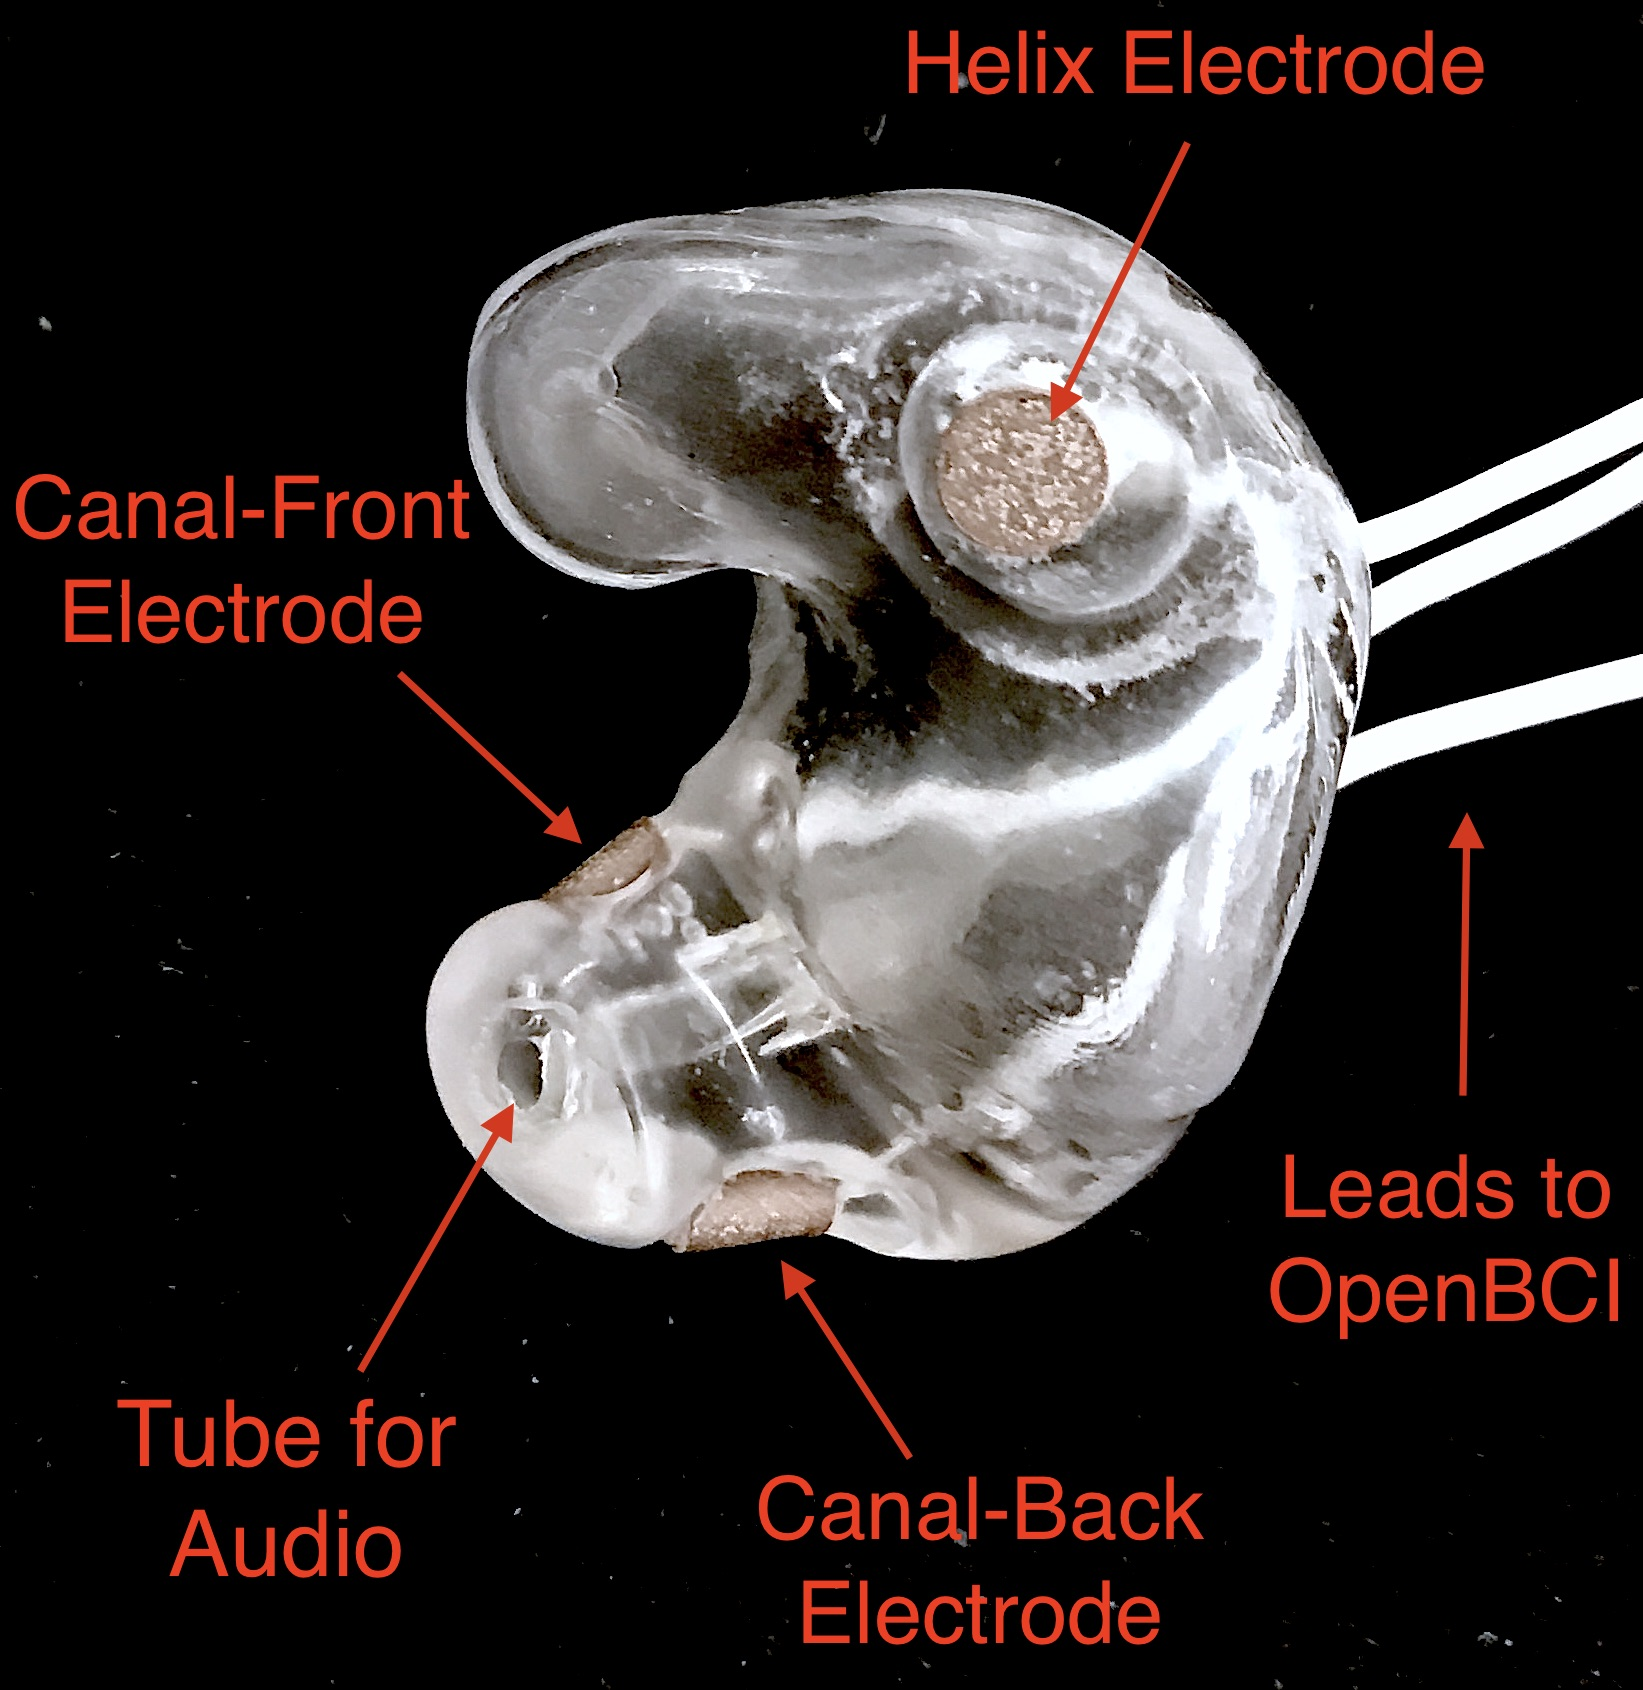
\includegraphics[width=.9\linewidth]{./figures/CFEEEG_piecefig_Right.jpg}
\caption{Labeled photo of one of our manufactured right ear custom-fit earpieces with 3 embedded electrodes located in the concha, and front-facing in the ear canal, and back-facing in the ear canal.}
\end{figure}

\subsection{In-Ear EEG}

Even consumer-grade headsets can be uncomfortable to wear, and are awkwardly visible to observers. Earbuds present a more discreet, comfortable location for an EEG sensor, as many people already wear earbuds in day-to-day life.

Research in in-ear EEG is only several years old. Nonetheless, the concept has
attracted a lot of attention because of the discreetness factor of in-ear EEG over
traditional scalp-based EEG. A research team at the Imperial College London
and Aarhus University published a landmark paper in 2011 that introduced the
concept of in-ear EEG, demonstrating for the first time the feasibility of recording
brainwave signals from within the ear canal
\cite{Looney2011}.
Follow-up work from the same
group demonstrated its ability to produce signal-to-noise ratios comparable to
those from conventional EEG electrode placements, robustness to common
sources of artifacts, and use in a brain-computer interface (BCI) system based on
auditory evoked potentials and visual evoked potentials
\cite{Looney2012a,Kidmose2013a,Kidmose2013b}.
United Sciences is currently developing a consumer "hearable'' (in-ear wearable) called The Aware, which will measure EEG from the ear, among other biometrics \cite{UnitedSciences}.

\cite{curranpassthoughts} was the first to merge in-ear EEG with passthought authentication,
 using a modified consumer grade EEG device with a single electrode, achieving approximately 80 percent authentication accuracy.

\section{Methods}

\subsection{Manufacturing and materials}

To produce custom ear impressions, we cleaned subjects' ears and injected silicon into the ear canal. A cotton ball with a string attached is placed into the ear canal first.  When the silicon dries after a few minutes, the string is pulled to remove the impression from the ear canal. This impression is then scanned with a 3D scanner and the resulting scan modified based on some heuristics to achieve a comfortable fit and to ensure the intended electrode sites will make good contact with the skin. Channels are created in the 3D model to allow wire leads and associated EEG electrodes as well as a plastic tube to deliver audio. This 3D model is then sent to a 3D printer. Following this wires leads and associated AGCL electrodes are installed. 

The electrode positions were simplified from the positions described in \cite{Mikkelsen2015}. We reduced the canal electrodes in order to help prevent bridging and positioned them approximately 180 degrees apart in the canal (posterior/back and anterior/front locations in the canal). We also reduced the number of electrodes in the concha to one.

\subsection{Study Overview}

7 male participants (P1-P7), 5 students and 2 non-students, completed our study protocol that was approved by our local Institutional Review Board. Three study visits took place per participant, in the first the 3D molds of participants' ears to use in creating the earpieces were obtained, the second to do a fit and electrical impedance check once earpieces were manufactured, and a third to collect data using the earpieces while participants performed a set of mental tasks to be used in authentication analysis. Informed consent was obtained prior to study procedures. The third study visit consisted of participants completing a short demographics questionnaire, a set up period with the OpenBCI system and earpieces including a second impedance check, the performance of 9 mental tasks presented on a laptop, and finally a post-experiment questionnaire. Approximately two weeks after the third study visit, a subset of participants reported via e-mail whether or not they remembered the passthoughts they chose and performed.

\label{sec:orgaf30da9}
\subsection{Tasks}

We used a set of mental tasks based on findings in related work regarding the relative strengths of different mental tasks in authentication accuracy and usability as reported by participants. Furthermore, given the in-ear placement of the electrodes and therefore the proximity to the temporal lobes containing the auditory cortex, we tested several novel authentication tasks based specifically on auditory imagery or stimuli. The 9 authentication tasks and their attributes are listed in Table \ref{tab:tasks}. Our strategy was to select tasks that captured a diversity of possibilities across the dimensions of external stimuli, involving a personal secret, eyes open or closed (due to known significant effects on EEG), and different types of mental imagery.

\begin{table*}[t]
\centering
%% \begin{tabular}{llllll}
\begin{tabularx}{\textwidth}{llllll}

\textbf{Task} & \textbf{Description} & \textbf{Stimuli}? & \textbf{Secret} ? & \textbf{Eyes} & \textbf{Imagery}\\
\hline
Breathe & Relaxed breathing with eyes closed & No & No & Closed & None\\
Breathe - Open & Relaxed breathing with eyes open & No & No & Open & None\\
Sport & Imagine acting out a sport-related task & No & Yes & Closed & Motor\\
Song & Imagine hearing a song & No & Yes & Closed & Aural\\
Song - Open & Song task, with eyes open & No & Yes & Open & Aural\\
Speech & Imagine a spoken phrase & No & Yes & Closed & Aural\\
Listen & Listen to noise modulated at 40 Hz & Yes & No & Closed & None\\
Face & Imagine a person's face & No & Yes & Closed & Visual\\
Sequence & Imagine face, a number, and word on timed cues & Yes & Yes & Open & Visual\\
\hline
\end{tabularx}
\caption{Properties of authentication tasks. We selected tasks with a variety of different properties, but preferred tasks that did not require external stimuli, as the need to present such stimuli at authentication time could present challenges for usability and user security.}
\label{tab:tasks}%
\end{table*}


\subsection{Data Collection Protocol}
\label{sec:org2041857}
The data collection visit took approximately 90 minutes for set up and experiment execution. All collection sites were cleaned with ethanol prior to electrode placement, and a small amount of conductive gel was used on each electrode. For EEG recording we used OpenBCI \cite{Frey2016}, an open-source biosensing system to maintain an overall low cost our set up. OpenBCI costs about \$600USD, and thus is an affordable alternative to medical-grade EEG systems that can cost tens of thousands of dollars. Recent work has demonstrated the robustness of OpenBCI compared to an industry standard medical-grade EEG system, particularly for non-medical use cases such as ours \cite{Frey2016}. The OpenBCI system we used allows for 8 channels of simultaneous recording, along with separate ground and reference channels. Data was collected with the ground placed at the center of the forehead, approximately AFz according to the 10-20 International Standard for Electrode Placement (ISEP), and using the left mastoid as reference. Notably, when examining data from the right earpiece, we re-referenced to the right mastoid channel so that our results reflect data from a single earpiece. Each earpiece (shown in Figure 1) contains three channels: one placed in the concha, and two inside the canal - one on the anterior canal wall (front-facing) and the other on the posterior wall (back-facing). The remaining two channels, AGCL ring electrodes, were placed on the right mastoid for later re-referencing, and at approximately Fp1 (left frontal lobe region, above the left eye in accordance with the ISEP) for validating the data collected in the ears against a common scalp-based placement. Before beginning the experiment, the data from each channel was visually inspected using the OpenBCI GUI and participants were asked to blink and clench their jaws to confirm that all channels were active and properly connected. Audio stimuli were delivered through small tubes in the earpieces opening into the ear canal.

During the experiment, participants were seated in a comfortable position in a quiet room facing a laptop screen on which the instructions and stimuli were presented using PsychoPy. Each task was completed once in sets five trials each, and then each was completed again for another five trials. Each trial was 10 seconds in length, for a total of 10 trials and 100 seconds of data collected per task. The instructions were read aloud to the participant by the experimenter, and the experiment was advanced using a pointer held in the participant's lap to minimize motion artifacts in the data. The experimenter also recorded the participant's chosen secrets for the sport, song, face, speech, and sequence tasks and reminded the participant of these for the second set of trials.
 
 After completing the experiment, a subset of participants completed a usability questionnaire asking about the ease of performing, level of engagement, perceived repeatability, and likeliness of using each task. The questionnaire also asked participants to rank the tasks overall from most to least favorite, as well as several open response questions regarding potential use cases of ear EEG and this method of authentication, level of comfort wearing the earpieces, and any other comments they chose to provide.

\section{Analysis}
\label{sec:org6c1a839}
\subsection{Data Validation}
\label{sec:org800f2bd}

In this section, we establish that the data we collected were of a neural origin, and had relatively little noise. We were able to confirm the custom-fit earpieces are able to collect EEG data using two tests: good impedances measured for the ear electrodes, and alpha-band activity attenuation when a participant's eyes were open versus closed.

The first quality check was examining the electrical impedances achieved for the ear pieces as a low impedance (<10 kOhm) 
is best for obtaining quality EEG signals. Table \ref{tab:impedances} below summarizes the impedances across the seven participants' six ear channels. With the exception of a few channels in select participants, impedances achieved were overall good. 

\begin{table}[h]
\begin{center}
\begin{tabular}{lrrrrrr}
& \multicolumn{6}{c}{\textbf{Impedances} [k\(\Omega\)]} \\
\cline{2-7}
& \multicolumn{3}{|c|}{\textbf{Left ear}} & \multicolumn{3}{c|}{\textbf{Right ear}} \\
\textbf{P} & \textbf{Concha} & \textbf{Front} & \textbf{Back} & \textbf{Concha} & \textbf{Front} & \textbf{Back} \\
\hline
1 & 4 & 4 & 4 & \textless1 & 4 & 3\\
2 & 9 & 5 & 4 & 3 & 4 & 4\\
3 & 4 & 5 & 4 & 9 & 6 & 9\\
4 & 4 & 5 & 4 & 3 & 16 & 9\\
5 & 9 & 20 & 7 & 3 & 7 & 9\\
6 & 5 & 8 & 2 & 1 & 1 & 9\\
7 & 2 & 9 & 8 & 7 & 5 & 6\\
\end{tabular}
\end{center}
\caption{Electrical impedances measured for earpiece electrodes.}
\label{tab:impedances}
\end{table}

Most of the recorded impedances of the earpiece electrodes were less than 5 k\(\Omega\), a benchmark used widely in previous
ear EEG work, and all except two were less than 10 k\(\Omega\). Nonetheless, the data from all electrodes were tested in the remaining two data quality tests.

For the alpha-attenuation test, data from the "Breathe" task was compared with that of the "Breathe - Open" task. It is a well-
known feature of EEG data that activity in the alpha-band (approximately 8-12 Hz range) increases when the eyes are closed
compared with a similar state with eyes open. For our participants, this attenuation is clearly visible even in just
a single trial's data. To further validate, we also performed this calculation on the data collected from the Fp1 electrode and see
the effect clearly here as well. The figure below shows the alpha attenuation in the left ear channels, as well as Fp1 of one participant as an example. We see the same effect in the right ear channels referenced to the right mastoid.

\begin{figure}[h]
\centering
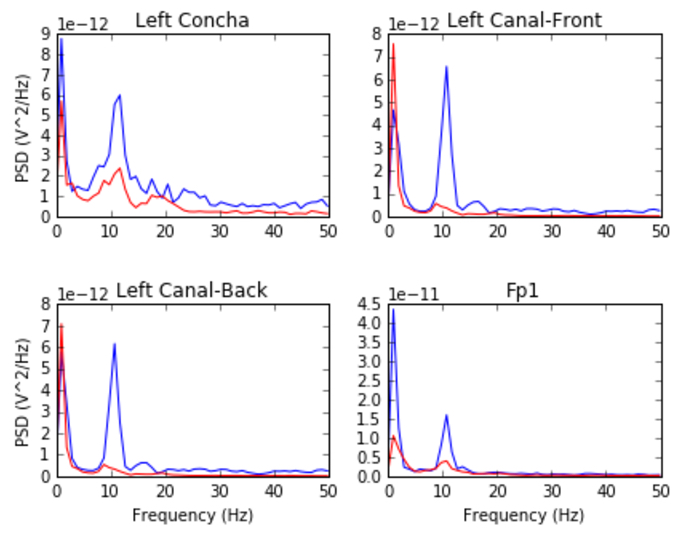
\includegraphics[width=0.5\textwidth]{figures/002_AlphaAtt_all.jpg}
\caption{Alpha-attenuation (8-12 Hz range) in left ear channels compared against the Fp1 channel, referenced at left mastoid. Red indicates breathing data with eyes open, blue indicates the same task with eyes closed.}
\end{figure}

\subsection{Classification}

We analyzed the EEG signals collected during the tasks using a support vector classifier (SVC). Since past work has shown that classification tasks in EEG-based BCI are linear \cite{Garrett2003a}, we used XGBoost, a tool for logistic linear classification \cite{Chen2016}. Compared to other linear classiifers, XGBoost uses gradient boosting; in which an algorithm generates an ensemble (in this case, a decision tree) of weak linear classifiers that minimizes a given loss function. Gradient boosting gives better results in linear classification problems, without our needing to manually tune classifier hyperparameters.

To produce feature vectors, we took slices of 100 raw values from each electrode (about 500ms of data), and performed an FFT to produce power spectra for each electrode during that slice. We concatenated all electrode power spectra together, and performed PCA on all concatenated vectors such that the resulting vectors described 95\% of the variance in the full power spectrum data. For each task, for each participant, 100 seconds of data were collected in total across 10 trials of 10 seconds each, resulting in 200 samples per participant, per task, following preprocessing.

We trained the classifier using a balanced sample of positive and negative examples, where positive examples were from the target participant and target task, and negative examples were randomly selected tasks from any participant besides the target participant.
From this corpus of positive and negative samples, we withheld one third of data for testing. 
The remaining training set was fed into a XGBoost's cross-validation method, which we set to iteratively tweak parameters over a maximum of fifty rounds of cross-validation to minimize loss.
After cross-validation, the updated classifier (with parameters applied) predicted labels on each sample in the test set, and we calculated FAR and FRR on its results.

\section{Results}
\label{sec:org6705b1d}
\subsection{Combinations of electrodes}
\label{sec:org21b14ae}

For each configuration of electrodes, we calculated the mean FAR and FRR across all participants using each task as the passthought (Figure \ref{fig:meanByElectrode}).
Incorporating all electrodes data results in a perfect score for all tasks.
Using data from all left-ear electrodes achieves the next lowest FAR, followed by all right ear electrodes.
Interestingly, no single electrode from the left or right ear performs as well as the aggregate left and right ear conditions. 
Counter to our expectations, Fp1 does not perform as well as most ear electrodes.

Our results indicate acceptable accuracy using electrodes on the left ear alone. 
This corresponds to our original scenario, in which the device could be worn as an earbud (ideally, only one earbud would need sensors).
As such, we focus on results from the left ear alone in our following analysis.

\begin{figure}[htbp]
\centering
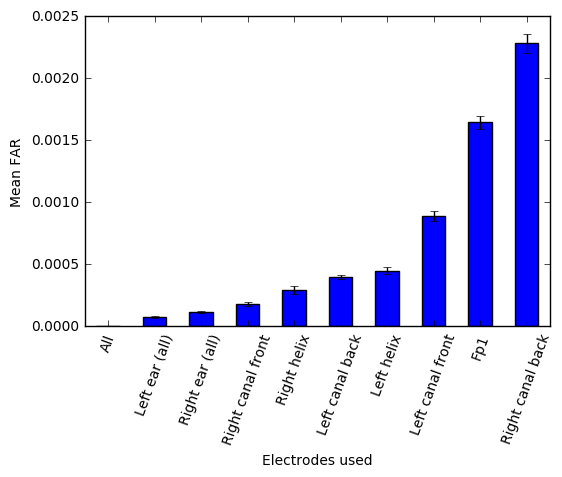
\includegraphics[width=.9\linewidth]{./figures/mean-far-by-electrode-config.png}
\caption{FAR by electrode configuration. All electrodes combined achieves a perfect score. We achieve the next best scores using data from the left ear only.}
\label{fig:meanByElectrode}
\end{figure}


\subsection{Authentication results in the left-ear}

In the previous section, we trained and tested a passthought classifier with each task as the passthought, for all participants. Focusing on the left ear, we filter our results for the best-performing tasks. We rank tasks by lowest FAR and, given a tie, the lowest FRR (Table \ref{tab:best}).

\begin{table}[h]
\begin{center}
\begin{tabular}{rrrl}
\textbf{P} & \textbf{FAR} & \textbf{FRR} & \textbf{Task}\\
\hline
1 & 0.0 & 0.0 & Listen\\
2 & 0.0 & 0.0 & Breathe\\
3 & 0.0 & 0.0 & Breathe\\
4 & 0.0 & 0.0 & Breathe\\
& 5 0.0 & 0.012 & Breathe\\
6 & 0.0 & 0.0 & Breathe\\
7 & 0.0 & 0.0 & Breathe\\
\end{tabular}
\end{center}
\caption{Best-performing passthought, with FAR and FRR, for each participant, using data from the left ear.}
\label{tab:best}
\end{table}

All best-performing tasks in our best-case set achieved perfect FAR and FRRs, with the exception of P5, whose best-performing task (breathe) had a nonzero FRR.
Breathe appeared as the best task across all participants. Given our training strategy, these results indicate that a given person's breathe task is distinguishable not only among other tasks, but among breathe tasks from other participants.
This task performed about as well as its open-eyes counterpart (Figure \ref{fig:meanByTask}), as did /Song (eyes open)/ and /sport/ (though, interestingly, song with eyes closed performed less well).

\begin{figure}[htbp]
\centering
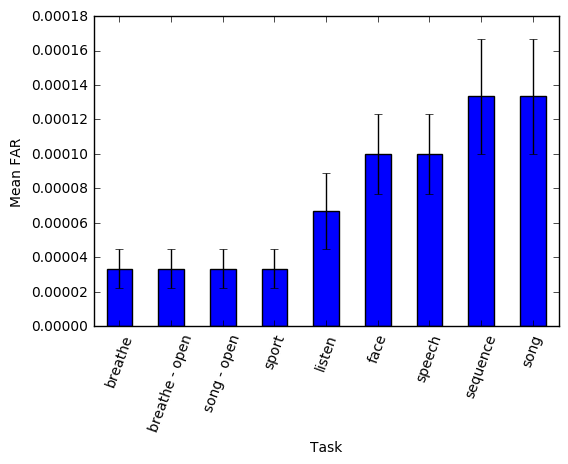
\includegraphics[width=.9\linewidth]{./figures/mean-far-by-task.png}
\caption{FAR in the left ear by task, across all subjects.}
\label{fig:meanByTask}
\end{figure}

These results establish good performance in our original training strategy, in which we count as negative examples recordings from the wrong participant performing any task. For comparison, we try two additional training strategies: one in which negative examples are the correct task recorded from the wrong participant (within-tasks), and one in which negative examples are the incorrect task recorded from the correct participant (within-participants).

\begin{table}[h]
\begin{center}
\begin{tabular}{lrr}
 & \textbf{FAR} & \textbf{FRR}\\
\hline
Original & 0.000074 & 0.004424\\
Within-tasks & 0.000724 & 0.001522\\
Within-participants & 0.002523 & 0.039702\\
\end{tabular}
\end{center}
\caption{Mean FAR and FRR for all participants and passthoughts across three different training strategies.}
\label{tab:compare}
\end{table}

Overall, our original training strategy achieves the lowest FAR (Table \ref{tab:compare}). Within-tasks FAR ten times higher, and within-participants FAR is one hundred times higher.
However, FRR is \textit{lower} in the within-tasks training strategy than in our original strategy's FRR. Within-participants again results in the highest FRR.

\subsection{Usability}

A subset of four participants completed our usability questionnaire. This questionnaire asked them to rank each of the mental tasks on 7-point likert-type scales on ease of use, level of engagement, perceived repeatability, and likeliness to use in a real-world authentication setting. The breathe and listen (\(\mu\)=6.75) tasks were ranked easiest to use, while the sequence (\(\mu\)=2.25) and face (\(\mu\)=2.75) tasks were ranked the most difficult. Sequence was rated highly in engagement however (\(\mu\)=5), as was the song task (\(\mu\)=5), while breathe-open and listen were ranked least engaging (\(\mu\)=2.25). Breathe (\(\mu\)=7) and listen (\(\mu\)=6.75) were ranked highest in repeatability, with sequence (\(\mu\)=2.5) along with face and sport (\(\mu\)=3) ranked least repeatable. Finally in terms of likeliness of use for authentication, song-open (\(\mu\)=5) and sequence (\(\mu\)=4.25) performed highest though modestly, while breathe (\(\mu\)=2.75) and listen (\(\mu\)=3) were rated least likely to use. In addition to these rating scales we asked participants to rank the tasks from most (1) to least (9) favorite overall. The song-open task ranked highest among favorites (\(\mu\)=4.25) followed by a tie between breathe-open, song, and speech (\(\mu\)=4.75). In line with some of the results above, sequence (\(\mu\)=7.75) and face (\(\mu\)=6.75) were rated as least favorites.

In addition to the scales and rankings, we included in our questionnaire a few open response questions to ascertain attitudes about the use cases for in-ear EEG and passthoughts, and the comfort of wearing an in-ear EEG device in everyday life. Participants first read the prompt, "Imagine a commercially available wireless earbud product is now available based on this technology that you've just experienced. It requires minimal effort for you to put on and wear.", and were asked about use cases for in-ear EEG and passthoughts. Responses about in-ear EEG expectedly included authentication for unlocking a phone or computer and building access, but also aspects of self-improvement such as P4's response "Help people increase focus and productivity". P5 and P6 also indicated a use for measuring engagement with media like movies and music, and relatedly P4 wrote "music playback optimized for current mental state and feelings". In terms of comfort wearing such a device, participants generally responded they would be comfortable, though P5 and P6 stipulated only when they would otherwise be wearing something like earphones in their ears already. In response to an "any other comments" prompt, notably three participants pointed out the mental imagery of a face was difficult for them and some concerns about their ability to repeat tasks in the same exact way each time.

A final component of usability we measured was the ability of the participants to recall their specific chosen passthoughts for the song, sport, speech, face, and sequence tasks. Participants were contacted approximately two weeks after their data collection study visit and were prompted with these categories and asked to respond with what they remembered their choices being. As evidenced by their responses, all participants were able to recall all of their chosen secrets, with the exception of one participant who incorrectly remembered their chosen word for the sequence task. 

\section{Imposter attack}

While our left-ear results establish that passthoughts achieve low FAR and FRR when tested against other participants' passthoughts, we do not know how robust passthoughts are against a spoofing attack, in which both a participant's custom-fit electrode, and details of that participant's chosen passthought, are leaked. 

The first aspect of this scenario we tested was the ability of an imposter to wear an earpiece acquired from someone else and achieve viable impedance values for EEG collection. P1 tried on each of the other participants' earpieces, which firstly were able to fit at least somewhat in P1's ears. The impedances of P1 wearing other participants' earpieces were then recorded and are listed in Table \ref{tab:imposter_impedances} below.

\begin{table}[h]
\begin{center}
\begin{tabular}{lrrrrrr}
& \multicolumn{6}{c}{Impedances [k\(\Omega\)]} \\
\cline{2-7}
& \multicolumn{3}{|c|}{\textbf{Left ear}} & \multicolumn{3}{c|}{\textbf{Right ear}} \\
\textbf{P} & \textbf{Concha} & \textbf{Front} & \textbf{Back} & \textbf{Concha} & \textbf{Front} & \textbf{Back} \\
\hline
2 & 34.1 & 10.2 & 12.8 & 27.8 & 16.0 & 16.3\\
3 & 21.1 & 20.9 & 19.0 & 13.5 & 11.3 & 19.5\\
4 & 14.1 & 11.9 & 9.7 & 11.0 & 11.1 & 13.3\\
5 & 17.2 & 21.9 & 10.3 & 32.6 & 12.5 & 11.6\\
6 & 18.7 & 10.0 & 8.4 & 14.8 & 11.5 & 8.9\\
7 & 91.5 & \textgreater1000 & 21.5 & 33.5 & 26.4 & 31.0\\
\end{tabular}
\end{center}
\caption{Electrical impedances measured while P1 wore each other participant's custom-fitted earpieces.}
\label{tab:imposter_impedances}
\end{table}

To explore the scenario of an imposter attempting to gain access, we chose the worst case participant, P6, whose earpieces P1 had the lowest impedances wearing. We collected data using the same data collection protocol, but had P1 refer to P6's report of chosen passsthoughts.
P1 performed each of P6's passthoughts (simulating an ``inside imposter''). Following the same classification and preprocessing steps, we generated 200 samples per task for our imposters, using data from all left ear electrodes.

\begin{table}[h]
\begin{center}
\begin{tabular}{lll}
Task & FAR (Insider) & FAR (Outsider)\\
\hline
Breathe & 0.0 & 0.0\\
Breathe - Open & 0.0 & 0.0\\
Sport & 0.0 & 0.0\\
Song I & 0.0 & 0.0\\
Song - Open & 0.0 & 0.0\\
Speech & 0.0 & 0.0\\
Listen & 0.0 & 0.0\\
Face I & 0.0 & 0.0\\
Sequence & 0.0 & 0.0\\
\end{tabular}
\end{center}
\caption{False acceptance rate for spoofed versions of P6's passthoughts, performed by an inside imposter (P1 from the original participant pool) and an outside imposter (not from the original participant pool).}
\label{tab:imposter}
\end{table}

Since every participant has one classifier per task (for which that task is the passthought), we are able to make 200 spoofed attempts with the correct passthought on each of P6's classifiers (Table \ref{tab:imposter}). We find no successful spoof attempts for tasks with a chosen secret (e.g., song, face). However, we also do not find any successful spoof attacks for tasks with no chosen secret (e.g., breathe). In all 1,800 spoof attempts (200 attempts for each of the 9 classifiers), we do not find a single successful attack on any of P6's classifiers.

However, since this participant's data appeared in the initial pool, the classifier may have been trained on his or her recordings as negative examples. To explore the efficacy of an outsider spoofing recordings, we repeated the same protocol with an individual who did not appear in our initial set of participants (an ``outside imposter,'' Table \ref{tab:imposter}). Again, we do not find any successful authentication attempts.

\section{Discussion}

Our findings demonstrate the apparent feasibility of single earpiece, achieving good results with only three electrodes and a reference, all on the left ear. FARs and FRRs are low across all participants and tasks, with FARs overall lower than FRRs. Participants' best-performing passthoughts typically seeing no errors in our training. Furthermore, no spoofed attacks were successful in our cursory analysis.

The powerful interactions between inherence and knowledge emerged in our spoofing attack. Although our target participant documented their chosen passthought, the spoofers found ambiguity in how these passthoughts could be expressed. For the face task, the spoofers did not know the friend the original participant had chosen. For the song tasks, though the song was known, the spoofers did not know what part of the song the original participant had imagined, or how it was imagined (humming, imagining a full performance, melody, vocals, etc). This experience sheds light on the highly individual nature of passthoughts, and provides a positive indication that there may be some intrinsic difficulty ofr spoofing passthoughts.

In our analysis, some notable patterns emerged. First, \textit{breathe} tended to be the best-performing task among participants. Classifiers overall distinguished the breath task even compared to breath tasks from other participants, implying that the task is expressed differently for each participant, i.e. that this task has an inherence factor sufficient for authentication, even though the task does not have a knowledge factor. Second, we were able to achieve good results by generating feature vectors based on only 500ms (300 voltage readings across the three electrodes). This short timespan is somewhat surprising, given that some tasks (like songs) presumably rely on changes or patterns over a longer period of time. 

Furthermore, the use of conductive gel results in low impedances on other participants' custom-fit earpieces, despite the uniquness of ear canal shapes between individuals \cite{Akkermans2005}.
Nevertheless, classifiers appear to resists spoofing attacks, indicating that task-related signals are unique to individuals.
In the future, the custom-fit earbuds could include a hardware keypair to sign authentication attempts, providing a more secure method for establishing the posession factor in our three-factor, one-step scheme.

Finally, performance on Fp1 was not as high as performance in the ear, despite Fp1's popularity in past work on passthoughts \cite{Chuang2013b}. This could be explained by the greater number of electrodes in the ear (compared to just one on Fp1). Additionally, Fp1 is best poised to pick up on frontal lobe activity (e..g, concentration), but our tasks did not generally involve frontal lobe activity; in fact, a good number of them involved audio, which we would expect to be better observed near the auditory cortex at the ears. Future work should continue to investigate what sorts of mental tasks lend themselves to in-ear recording.

\section{Future Work}

One primary question surrounds how our passthought system performance will change with a greater number of users, and with more diverse data. Our system specifically trains on negative examples of non-users; we do not yet know how this approach will scale. At the same time, we must investigate the stability of EEG readings for a passthought are over time. We must also collect EEG data from the variety of different user states: ambulatory settings, during physical exertion or exercise, under the influence of caffeine or alcohol, etc.

% We provide cursory evidence that passthoughts are difficult to spoof, though further work should expand on ours with more subjects.
Another important question surrounds how passthoughts might be cracked.
Generally, we do not understand how an individual's passthought is drawn from the distribution of EEG signals that an individual produces throughout the day. 
Given a large enough corpus of EEG data, are some passthoughts as easy to guess as \textit{password1234} is for passwords?
Future work should perform statistical analysis on passthoughts, such as clustering (perhaps with t-SNE) to better understand the space of possible passthoughts.
This work will allow us simulate cracking attempts, and to develop empirically motivated strategies for prevention, e.g. locking users out after a certain number of attempts.
This work could also reveal interesting tradeoffs between the usability or accuracy of passthoughts and their security.

Finally, our work leaves room for some clear UX improvements.
Future work should try using dry electrodes, commonly found in consumer EEG devices, for comfort and usability.
Future work should also attempt a closed-loop (or online) passthought system, in which users receive immediate feedback on the result of their authentication attempt. A closed-loop BCI system could help us understand how learning effects
on the human side might impact authentication performance, as the human and machine co-adapt through authentication attempts.

\section{Conclusion}

We believe custom-fit, in-ear EEG earbuds could provide three factors of authentication in a authentication single step: thinking one's password. In this paper, we demonstrate quite high authentication accuracy using a single sensing earbud. By expanding our corpus of EEG readings (in population size, time, and diversity of settings), we hope to better understand the underlying distribution of EEG signals, so that we may better understand the security properties of passthoughts.

{\footnotesize \bibliographystyle{acm}
\bibliography{references}}


\end{document}
